\documentclass[twocolumn]{article}
\usepackage{titling}
\usepackage{listings}
\usepackage{xcolor}
\usepackage{graphicx}
\usepackage{geometry}
\usepackage{hyperref}

\geometry{margin=1in}
\lstset{ 
    language=C++,
    tabsize=2, % sets default tabsize to 2 spaces
    basicstyle=\footnotesize,% basic font setting
    breaklines=true, % sets automatic line breaking
}


\begin{document}
\title{Project 2B}
\author{Jordan Lynn}
\date{10/16/2015}
\maketitle
This project was influenced by Dr. Terry Soule's code found here \url{http://www2.cs.uidaho.edu/~cs472_572/f15/GPProjectA.html} while not an exact copy, some of the program flow was referred to. This project is also in C++ so this made things go faster and more smoothly.

\section{Initialization}
From the beginning the population, amount of generations and the tournament sizes are all decided in a few local \#define parameters at the top of main.cpp. As parts of this program are fine tuned this is where most the alterations happen. The program first generates an array of individuals from the ``individual'' class. A for loop creates each individual with a random tree depth in the range of $4->7$. Through testings and the hardware limitations of the testing computer this seemed to be a nice optimum between balancing needed complexity and limited system resources.

Once the individuals have been generated they are immediately evaluated. The evaluation function is an important subroutine withing this program because the function will do things not only like assigning fitness but also finding tree depth and size as well as other important information. So after each individual undergoes changes you'll often see a call to evaluation to get info about the new individual.

There is some additional file I/O going on throughout, while not critical and only for data gathering it is worth mentioning it's built in, and it is going to be required for use in future projects.

Once the evaluation is done the first tournament is started. The tournament size itself is \#define in the beginning of main.cpp, when using this program the user has to make sure this number is divisible by two because of how the tournament works. If an odd number is used your last individual is never crossed over, while not critical or program crashing this could cause discrete problems if a user isn't aware the last odd individual isn't being used. Once the tournament is over the program will take some data/statistics from the information and new individuals in the population and check if it has anymore ``Generations'' to do. While this program doesn't use a generational model the term generation is used to identify a full cycle of: Evaluate$\rightarrow$Get populations' fitness$\rightarrow$Tournament. Once the generations are over the individual's tree with the best fitness is printed.

\section{Tournament}
The tournament function is found in main.cpp and takes in the array of the population as a parameter. ``tournament()'' then creates a second array of pointers of individuals named ``individual *tributes[TOURNYSIZE];'' that is used to keep track of those partaking in the tournament. A ``for()'' loop then starts off by pointing the tributes at any random individual in the population. Using a ``do{}while()'' loop withing the ``for()'' loop to make sure that no two pointers are referencing the same individual. This algorithm can be found on the final page of this document. The tributes are then sorted by their fitness values using C++11's ``sort()'' function which is capable of sorting an array of objects based on a given parameter within those objects. A final ``for()'' loop then begins crossover starting with the best individual at the beginning of the tributes array and crossing it with the individual next to it in the array.

\section{Crossover}
Crossover of two trees from an individual happens within the ``individual'' class. The function itself is defined as ``CrossOver(individual *toMate){}'' as you can see the better individual is passed a pointer to the individual next to it in the tournament. The function then creates two more individuals using C++11's ``unique\_ptr'' as the pointer to these new individuals. This is to help with cleanup and garbage collection. These individuals are made as exact copies of the original tribute individuals. Then a random node is pointed to in one tree and the same for the ``*toMate'' individual and swapping at these two points is done. This code follows below.
\begin{lstlisting}[frame=single]
// Two random points in the two trees.
node *nodePoint = holder->rootNode->RandomCross(holder->rootNode, rand()%1+holder->depth);
node *nodePointTwo = holder2->rootNode->RandomCross(holder2->rootNode, rand()%1+holder2->depth);

nodetmpParent = nodePoint->parent;
node2tmpParent = nodePointTwo->parent;

if(nodetmpParent->branch[0] == nodePoint)
	nodetmpParent->branch[0] = nodePointTwo;
else
	nodetmpParent->branch[1] = nodePointTwo;
nodePointTwo->parent = nodetmpParent;

if(node2tmpParent->branch[0] == nodePointTwo)
	node2tmpParent->branch[0] = nodePoint;
else
	node2tmpParent->branch[1] = nodePoint;
nodePoint->parent = node2tmpParent;
\end{lstlisting}
These individuals are then mutated and compared to their parents. If the children do not score a better fitness (calculated as the RMS error of a mathematical function) then they are discarded, if they are better they are ``AntiSelected'' back into the population via pointing the old tribute's pointers at the new crossed over individuals.

\section{Mutation}
Mutation is simple and fast, the mutation function is apart of the ``node'' class and advances through the tree node-by-node and has a $10\%$ chance to mutate a given node.

\section{AntiSelect}
Once the tournament is over and we have new individuals ready and willing to replace the poorer scoring individuals the ``AntieSelect()'' function is called from the ``Tournament()'' function discussed above. AntiSelect takes in the population and the tribute arrays as parameters and creates another array of pointers named ``terribleIndividuaIndex'' which is the size of the population and is used to find the worst individuals. These pointers are pointed at each individual in the population and then as before we use C++11's ``sort()'' function and arrange these pointers to the population in reverse order of worst scores first and best scores last. The double nested ``for()'' loop below is the main algorithm at play in the antiselection step, and what it does is checks to see if it's crossed over individual is better than the ``terribleIndividualIndex'' and if so replaces that individual and continues for the rest of the tributes.

\begin{lstlisting}[frame=single]
for(int k=0; k < TOURNYSIZE; k++){
		for(int l=0; l < POP; l++){
		if(terribleIndividuaIndex[l]->GetFitness() > tributes[k]->GetFitness()){
		terribleIndividuaIndex[l]->rootNode = tributes[k]->rootNode;
		terribleIndividuaIndex[l]->Evaluate();
		break;
		}
	}
}
\end{lstlisting}
\section{Results \& Conclusion}
As of now everything seems to be working as a GA should. Below is a graph showing the fitness improving when the program is given the function $((x_1 * 2)*(x_2+1) - x_2^2 + 5*x3 +x_3^3 +5)$. Right now the only limitation seems to be the personal laptop I'm running the program on. Often you can see me crossing my fingers watching my RAM usage inch closer to 100\% as the trees grow. I will need to implement some type of control for this. Additionally I'd like to play with the idea of making the algorithm aware of how much of the system's resources it's using and take that amount into account when calculating fitness. More works is needed to show if this is viable however.
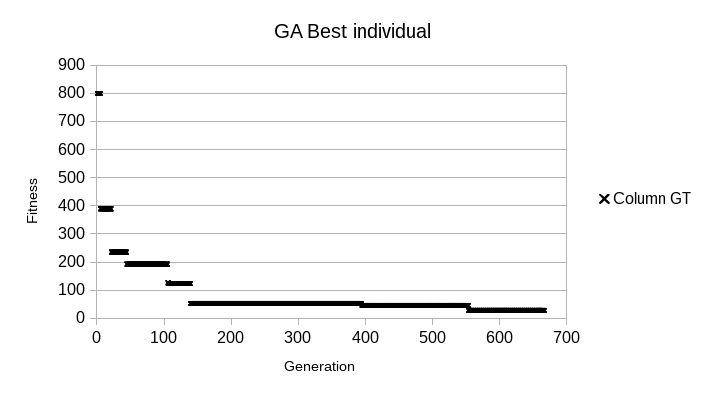
\includegraphics[width=9.5cm]{graph.png}

\pagebreak
\onecolumn
\begin{lstlisting}[frame=single]
void Tournament(individual population[POP]){
	individual *tributes[TOURNYSIZE];
	int index[TOURNYSIZE];
	int* found;
	bool iterate = false;

	for(int l=0; l < TOURNYSIZE; l++)
		index[l] = -1; // Initialize array

	// Now fill copetitor positions.
	for(int i=0; i < TOURNYSIZE; i++){
		do{
			iterate = false;
			index[i] = rand()%POP;
			for(int j=0; j < i; j++){
				if(index[i] == index[j])
					iterate = true;
			}
		}while(iterate);
		tributes[i] = &population[index[i]];
		iterate = true;
	}

	// Now sort the tributes array!
	sort(begin(tributes), end(tributes), [](individual* a, individual* b) { return a->GetFitness() < b->GetFitness(); });

	for(int k=0; k < (TOURNYSIZE/2); k++)
		tributes[k]->CrossOver(tributes[k++]);

	AntiSelect(population, tributes);
}
\end{lstlisting}
\end{document}

